\chapter{\GP Performance Testing}
\label{chap:GPtesting}

Before installation all of the \GP fibers were tested for throughput
performance using the Wisconsin Test Stand
\citep{Bershady04,Crause08,Eigenbrot12}. This stand is a
double-differential imaging comparator. It consists of an input stage
that reimages an illuminated aperture through a controllable aperture
at an intermediate pupil, and an output stage that consists of a
collimator that places the output pupil from the reimager or fiber
output onto a CCD detector. The experiment consists of measuring the
input beam differentially between a straight-through configuration and
the collimated fiber output. During the entire process the stability
of the filtered input beam is monitored with a photo diode.

Tests were performed in the Johnson $V$ band with an input beam set to
match the WIYN input beam of $f$/6.3 without the 17\% central
obstruction of the telescope. The total throughput ($T_{\rm tot}$) is
defined as all of the fiber-output light captured by the CCD (roughly
corresponding to $f$/2.2, compared with the fiber numerical aperture
of $f$/2.3)
%From 54mm L3 / 1024px * 0.024mm/px. NA = 0.22 and N = (2*arctan(NA))^-1
divided by the all of the light from the input beam captured by the
same CCD. This gives a good indication of the total transmission
through the fiber, but ignores the effects of FRD on the delivered
throughput on the Bench Spectrograph due to the optical stops
therein. FRD describes the tendency for fibers to increase the entropy
in an optical beam; light injected into a fiber at a particular
$f$-ratio emerges at a smaller (faster) $f$-ratio \citep{Angel77}.

The primary impact of FRD is from light loss from obstructions inside
the Bench Spectrograph as detailed in \cite{Bershady04} and
\cite{Bershady05}.  With the upgrade \citep{Bershady08} the low-order
gratings and camera objective are sufficiently near the pupil and are
of sufficient size that the limiting stop is from the collimator. The
camera objective does begin to vignette for off-axis fields point in
wavelength and pseudo-slit position, but for operational purposes we
consider the on-axis field point for defining throughput losses due
to FRD.  The collimator accepts light up to $f$/4 with only minimal
obstruction, and is completely unobstructed at $f$/4.4, while the
optical design (in terms of aberrations) is optimized for f/5.

To characterize the impact of FRD on the the delivered throughput we
define the quantity
\begin{equation}
\label{GPtesting:eq:T_FRD}
  T_{\mathrm{4}} = \frac{F_{\mathrm{out}}(f<f/4)}{F_{\mathrm{in}}(f<f/6.3)},
\end{equation}
where $F_\mathrm{in}$ and $F_\mathrm{out}$ represent flux from the the
input and fiber output beams, respectively. $T_4$ is essentially a
throughput measurement that accounts for the impact of FRD, and should
be representative of how the fibers will perform as part of the
WIYN/Bench system.  We compute comparable quantities for output
f-ratios of f/4.5 and f/5.  The throughput in each of these apertures,
as well as the total throughput are included in Table
\ref{GPtesting:tab:GP_cal_full} as $T_{\rm tot}$, $T_4$, $T_{4.4}$,
$T_{5}$.

\begin{figure*}[htb]
  \centering
  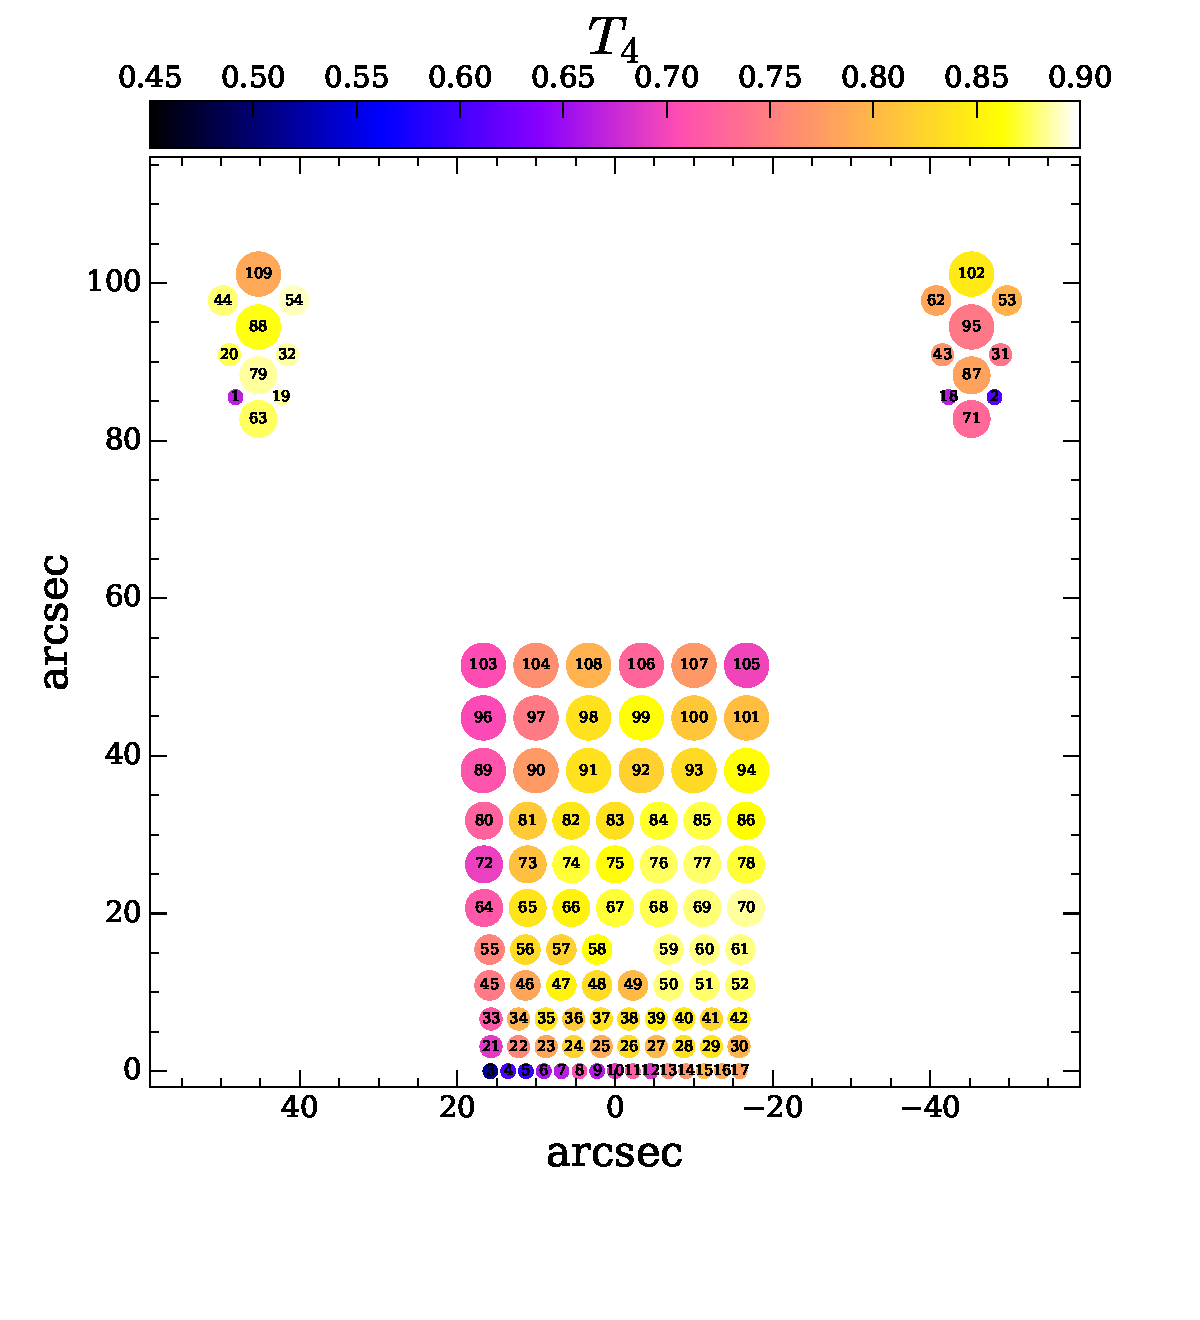
\includegraphics[width=0.4\textwidth]{Appendix/figs/gradpak_map.pdf}
  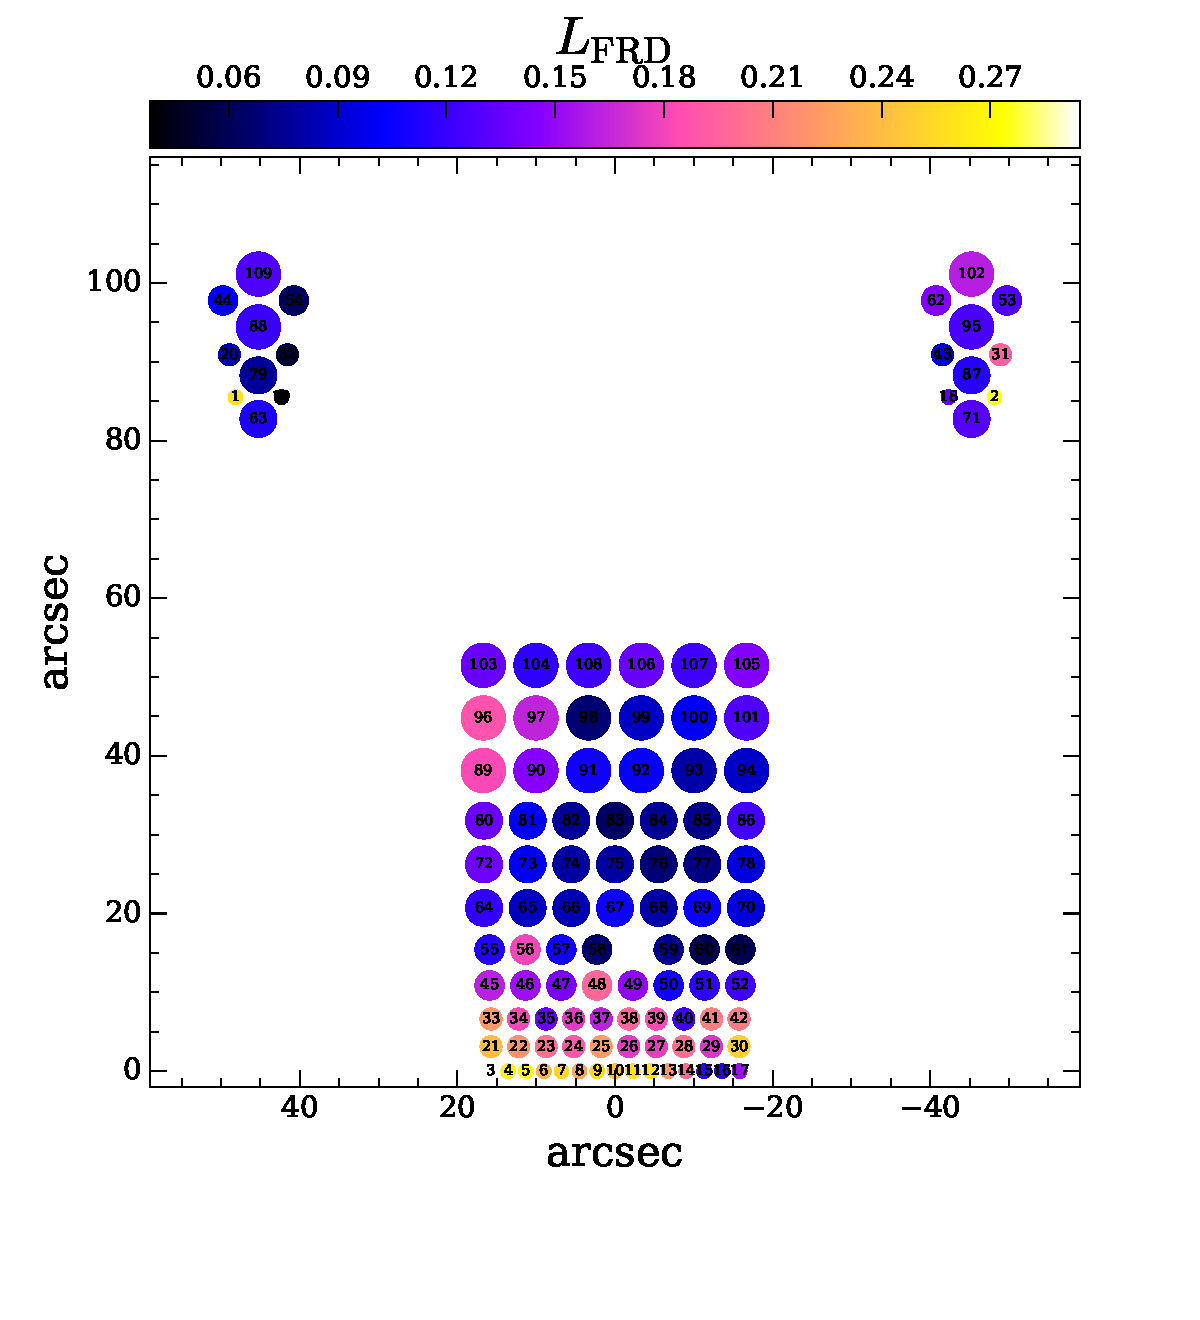
\includegraphics[width=0.4\textwidth]{Appendix/figs/gradpak_L_map.pdf}
\vskip -0.25in
\caption[\GP throughput and and FRD
losses]{\label{GPtesting:fig:TL_FRD}\fixspacing Maps of laboratory
  measurements of the \GP IFU performance. Throughput
  ($T_{\mathrm{FRD}}$, Equation \ref{GPtesting:eq:T_FRD}) is shown in
  the left-hand panel, while throughput losses ($L_{\mathrm{FRD}}$,
  Equation \ref{GPtesting:eq:L_FRD}), is shown in the right-hand
  panel. Performance values are given in the color scale at the top of
  each panel.}
\end{figure*}

\begin{figure}
  \centering
  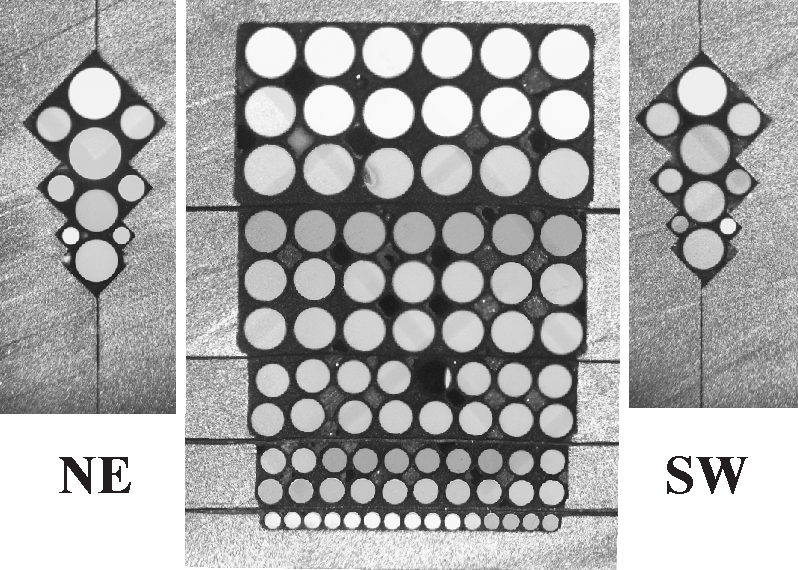
\includegraphics[width=0.8\textwidth]{Appendix/figs/gradpak_facefig.pdf}
  \caption[\GP face and polishing
  detail]{\label{GPtesting:fig:gradpak_face}\fixspacing Detail of \GP
    fiber face
    after polishing. The \val{25.4}{\mu m} (0.24'') shims between each
    block fiber-size group are visible in the central array. The hole
    in the 5th fiber row from the bottom is a fiber that was broken
    during polishing. The two sky-fiber groups, not shown to scale,
    have locations marked in Figure \ref{891_1:fig:GradPak}.  The
    \val{200}{\mu m} (1.87'') sky fibers are not visible in this image
    due to imperfect illumination conditions at the slit end when this
    picture was taken.}
\end{figure}

Figure \ref{GPtesting:fig:TL_FRD} contains throughput measurements for all of
the active \GP fibers. Throughput losses caused by FRD are spatially
coherent and are larger on the top and left (North and East) side of
the IFU. This is likely due to surface scattering at the IFU face
\citep{Eigenbrot12} caused by an uneven polish. Figure
\ref{GPtesting:fig:gradpak_face} shows evidence of this variable polish in the
two sky fiber groups; the SW sky group show significantly worse polish
than the NE group and has a correspondingly lower throughput. It is
important to note that the FRD losses do \emph{not} appear to be
caused by edge fibers pushing against the aluminum structure, as
evidenced by the relatively high throughput seen on the left side of
the IFU. This is consistent with previous studies \citep{Bershady04}
that suspected removal from an IFU molding fixture to be the primary
cause of stress-induced FRD. Variations in polish quality appears to
be caused by detritus from the aluminum fixture.

As a check on the lab measurements of $T_4$ we also compare total
fiber transmission recorded during the observing program described in
\S\ref{891_1:sec:obs}. For these measurements a stitched dome flat (see
\S\ref{891_1:sec:flats} was used as a good approximation of a uniform
illumination at the fiber input. The total light transmitted by each
fiber is computed by adding together all wavelength channels for each
fiber after the data were spectrally extracted. Figure
\ref{GPtesting:fig:count_tput} shows are comparison between lab
($T_4$) and on-telescope performance. ``Counts'' in this figure are
from dome-flats combined as described in \S\ref{891_1:sec:flats}), and
are the sum across all wavelengths of the extracted fiber traces.  As
expected from Figure \ref{GPtesting:fig:TL_FRD} the highest
throughputs are found in the middle of the array, with a gradual drop
off in performance towards the end of the slit. The right panel of
Figure \ref{GPtesting:fig:count_tput} shows a tight correlation
between our lab measurements and the on-sky performance. This shows
that stresses during installation and the performance of the Bench
Spectrograph only cause a $\pm$5\% rms modulation in the throughput
compared to what was measured in the lab.

We also measure the magnitude of FRD experienced by each
fiber. Because FRD represents a scattering of input light to larger
output angles a comparison between throughput at two different output
$f$-ratios gives an approximation of the severity of FRD in each
fiber. We define
\begin{equation}
\label{GPtesting:eq:L_FRD}
  L_\mathrm{FRD} = 1 - \frac{T_5}{T_4},
\end{equation}
which quantifies the amount of light scattered to smaller $f$-ratios
(larger angles) than $f/5$ as a measure of the severity of FRD
experienced by each fiber.

\begin{figure*}
  \centering
  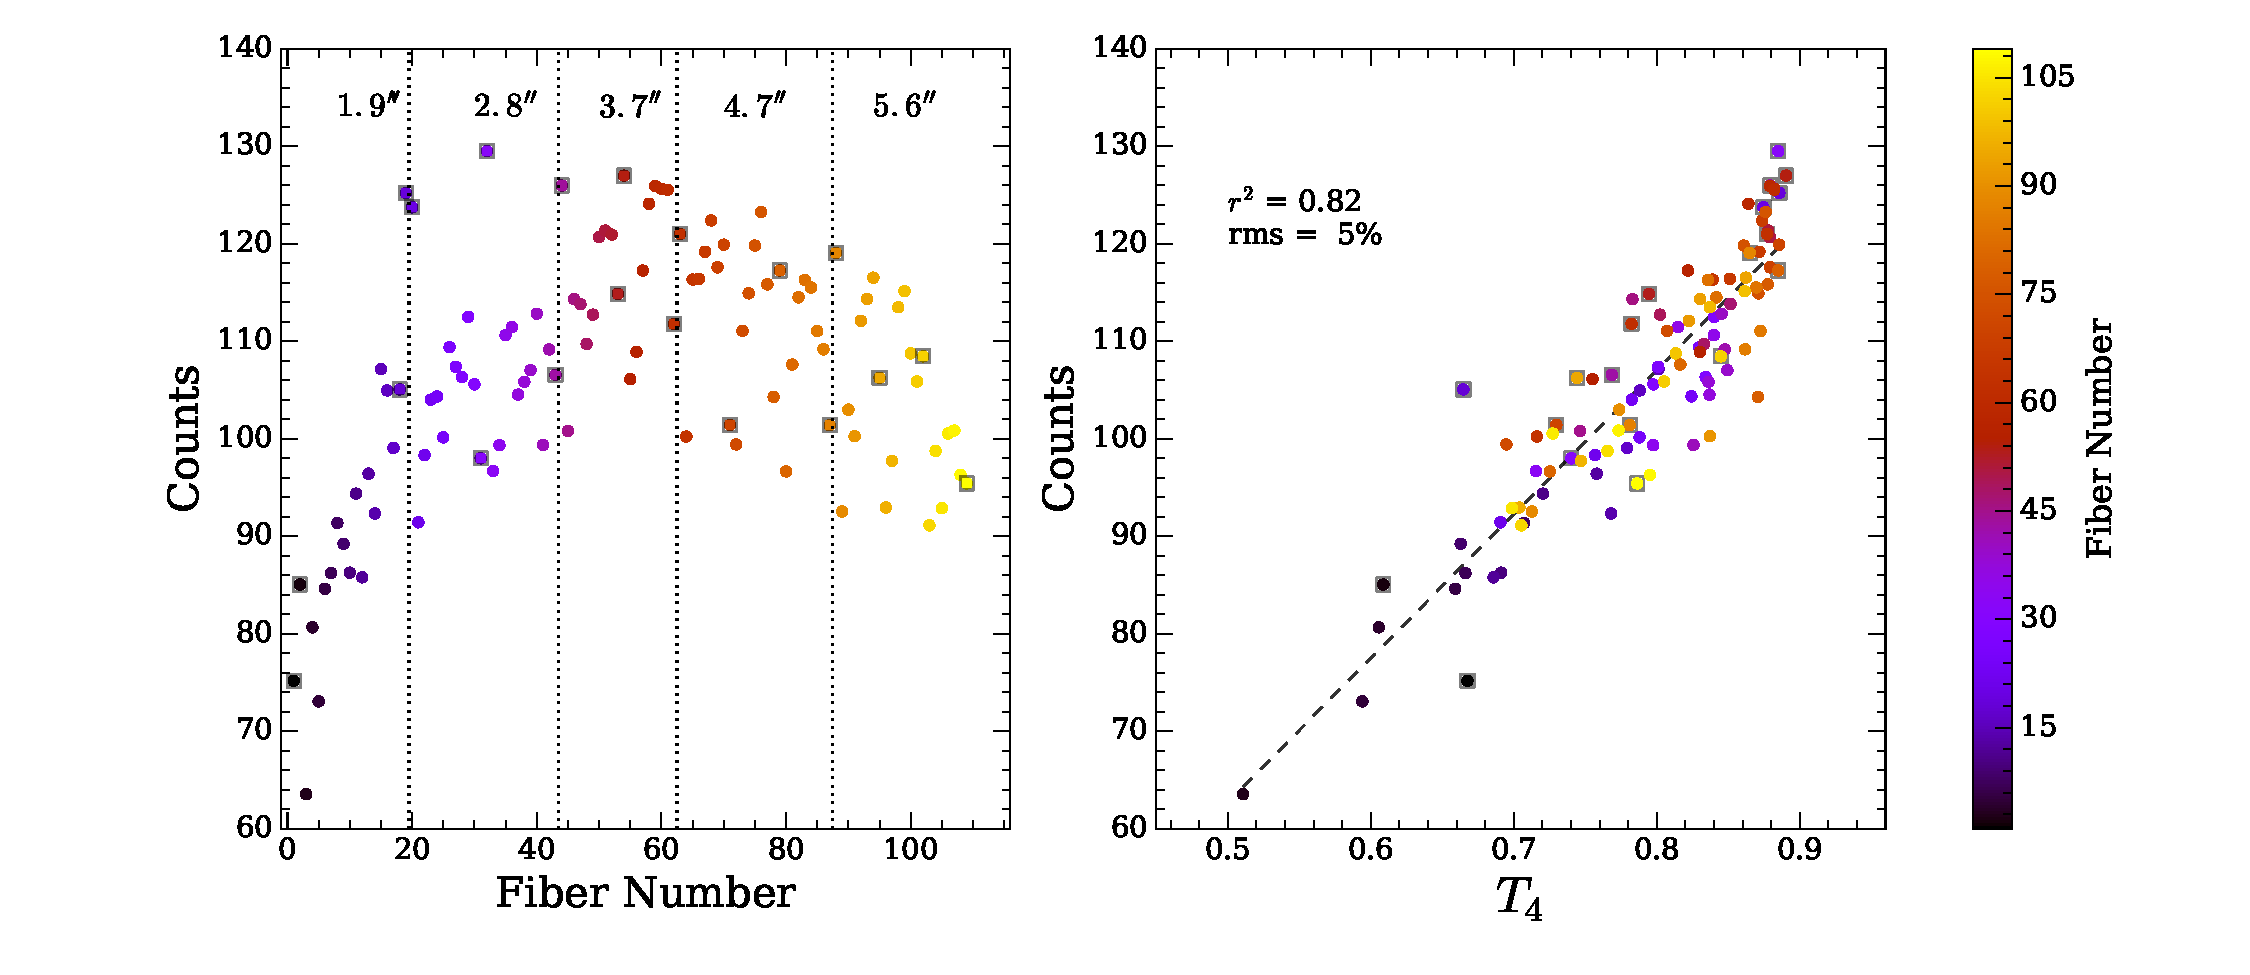
\includegraphics[width=\textwidth]{Appendix/figs/gradpak_count_plots.pdf}
  \caption[\GP on-bench throughput
  performance]{\label{GPtesting:fig:count_tput}\fixspacing Left:
    Relative fiber
    transmission measured \emph{in-situ} on the WIYN Bench
    Spectrograph. Vertical lines demark transition between different
    fiber sizes, as labeled. Right: Comparison between the
    \emph{in-situ} performance and $T_4$, as measured in the lab after
    construction. The dashed line represents a linear regression to
    the data with given correlation coefficient and scatter. Points
    are color-coded by fiber number (slit position), and sky fibers
    are marked with black squares.}
\end{figure*}

\begin{figure*}
  \centering
  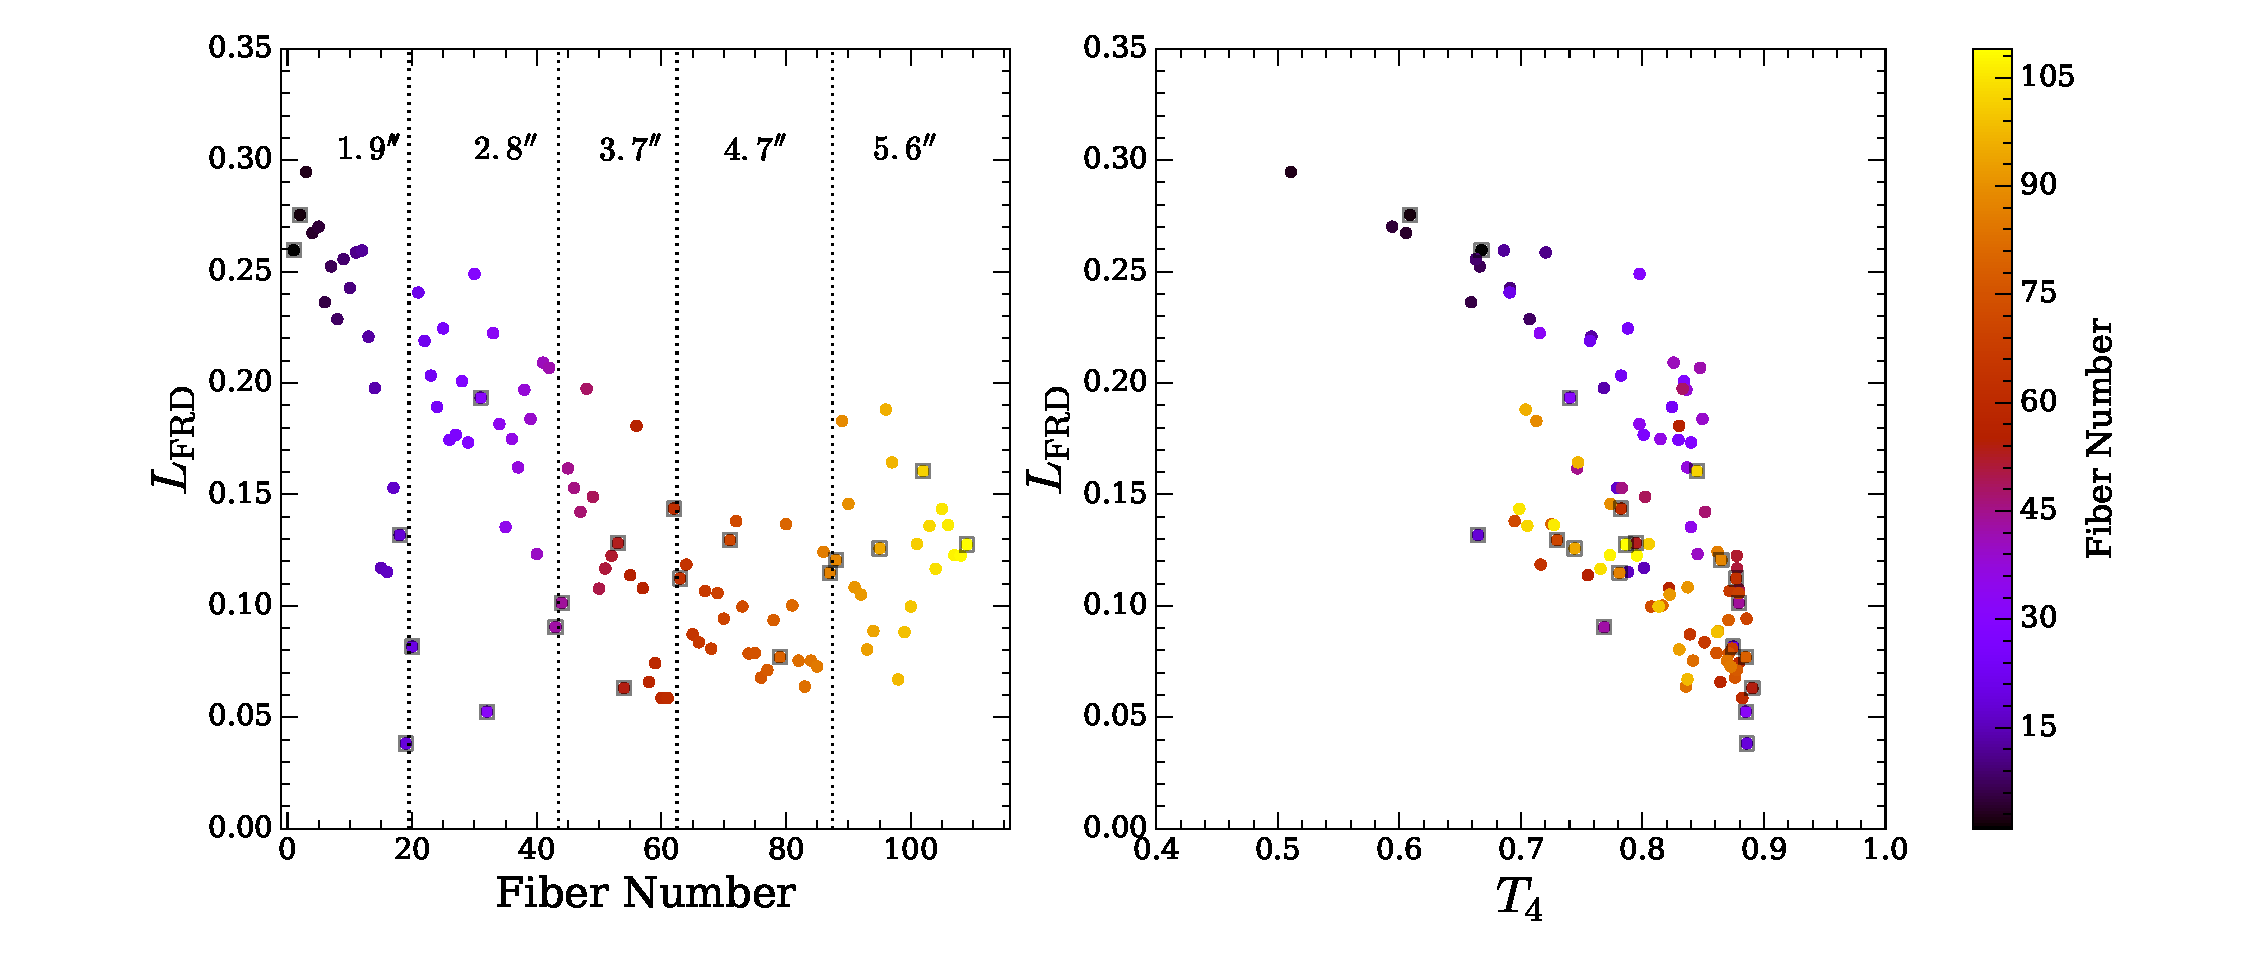
\includegraphics[width=\textwidth]{Appendix/figs/gradpak_Lplots.pdf}
  \caption[\GP on-bench FRD
  losses]{\label{GPtesting:fig:FRD_loss}\fixspacing Performance
    metrics for \GP. $L_\mathrm{FRD}$ (Equation
    \ref{GPtesting:eq:L_FRD}) as a function of slit location (right)
    and $T_4$ (transmission through an f/4 aperture). Points are
    color-coded by fiber number (slit position), and sky fibers are
    marked with black squares.}
\end{figure*}

Table \ref{GPtesting:tab:GP_cal_full} contains measurements and Figure
\ref{GPtesting:fig:TL_FRD} shows a map of $L_\mathrm{FRD}$ for each
\GP fiber. Figure \ref{GPtesting:fig:FRD_loss} compares this quantity
with $T_4$. We find that fibers with low $T_4$ also tend to have high
FRD losses ($L_\mathrm{FRD}$), which indicates that FRD is a
significant source of throughput loss in the \GP and Bench
Spectrograph system.  However this is relatively more pronounced for
smaller fiber sizes, as seen in the bifurcation in the right-hand
panel of Figure \ref{GPtesting:fig:FRD_loss}. Smaller fibers tend to
suffer from larger amounts of FRD, which may have been caused in \GP
due to handling-induced stresses; these fibers were more likely to
bend and tangle during construction.  The corollary is that lower
throughput in larger fibers isn't always the result of increased FRD.

A complete set of measurements showing FRD losses as a function of
output $f$-ratio for each fiber can be found in the supplemental
materials online. {\bf [can they? I'm thinking this would basically be
    a copy of what is available at
    \url{www.astro.wisc.edu/~eigenbrot/PAK} MAB: include material here
    since the www at the above address will not be archival.]}.

% \begin{deluxetable}{ccccc}
    \tablewidth{0.9\columnwidth}
\tablecaption{\GP Lab Data}
\tablehead{
    \colhead{Fiber} &
    \colhead{$T_\mathrm{tot}$} &
    \colhead{$T_4$\tablenotemark{a}} &
    \colhead{$T_{4.4}$} &
    \colhead{$T_5$} \\
    \colhead{Number} &
    \colhead{} &
    \colhead{} &
    \colhead{} &
    \colhead{}
}
\startdata
   1 &  0.84 &  0.67 &  0.58 &  0.49 \\
   2 &  0.78 &  0.61 &  0.53 &  0.44 \\
   3 &  0.75 &  0.51 &  0.44 &  0.36 \\
   4 &  0.75 &  0.61 &  0.53 &  0.44 \\
   5 &  0.76 &  0.59 &  0.52 &  0.43 \\
   6 &  0.77 &  0.66 &  0.59 &  0.50 \\
  %%    7 &  0.79 &  0.67 &  0.59 &  0.50 \\
  %%    8 &  0.79 &  0.71 &  0.64 &  0.55 \\
  %%    9 &  0.77 &  0.66 &  0.59 &  0.49 \\
  %%   10 &  0.78 &  0.69 &  0.62 &  0.52 \\
  %%   11 &  0.80 &  0.72 &  0.64 &  0.53 \\
  %%   12 &  0.77 &  0.69 &  0.61 &  0.51 \\
  %%   13 &  0.82 &  0.76 &  0.69 &  0.59 \\
  %%   14 &  0.80 &  0.77 &  0.71 &  0.62 \\
  %%   15 &  0.81 &  0.80 &  0.78 &  0.71 \\
  %%   16 &  0.80 &  0.79 &  0.76 &  0.70 \\
  %%   17 &  0.80 &  0.78 &  0.74 &  0.66 \\
  %%   18 &  0.73 &  0.66 &  0.64 &  0.58 \\
  %%   19 &  0.86 &  0.89 &  0.88 &  0.85 \\
  %%   20 &  0.85 &  0.87 &  0.86 &  0.80 \\
  %%   21 &  0.76 &  0.69 &  0.62 &  0.52 \\
  %%   22 &  0.81 &  0.76 &  0.69 &  0.59 \\
  %%   23 &  0.82 &  0.78 &  0.72 &  0.62 \\
  %%   24 &  0.84 &  0.82 &  0.77 &  0.67 \\
  %%   25 &  0.83 &  0.79 &  0.72 &  0.61 \\
  %%   26 &  0.83 &  0.83 &  0.79 &  0.68 \\
  %%   27 &  0.83 &  0.80 &  0.75 &  0.66 \\
  %%   28 &  0.85 &  0.83 &  0.78 &  0.67 \\
  %%   29 &  0.85 &  0.84 &  0.79 &  0.69 \\
  %%   30 &  0.85 &  0.80 &  0.72 &  0.60 \\
  %%   31 &  0.80 &  0.74 &  0.69 &  0.60 \\
  %%   32 &  0.86 &  0.89 &  0.88 &  0.84 \\
  %%   33 &  0.78 &  0.72 &  0.65 &  0.56 \\
  %%   34 &  0.82 &  0.80 &  0.74 &  0.65 \\
  %%   35 &  0.84 &  0.84 &  0.80 &  0.73 \\
  %%   36 &  0.83 &  0.81 &  0.76 &  0.67 \\
  %%   37 &  0.84 &  0.84 &  0.79 &  0.70 \\
  %%   38 &  0.85 &  0.84 &  0.78 &  0.67 \\
  %%   39 &  0.85 &  0.85 &  0.80 &  0.69 \\
  %%   40 &  0.84 &  0.85 &  0.82 &  0.74 \\
  %%   41 &  0.85 &  0.83 &  0.76 &  0.65 \\
  %%   42 &  0.86 &  0.85 &  0.79 &  0.67 \\
  %%   43 &  0.79 &  0.77 &  0.75 &  0.70 \\
  %%   44 &  0.85 &  0.88 &  0.86 &  0.79 \\
  %%   45 &  0.77 &  0.75 &  0.71 &  0.63 \\
  %%   46 &  0.81 &  0.78 &  0.74 &  0.66 \\
  %%   47 &  0.85 &  0.85 &  0.82 &  0.73 \\
  %%   48 &  0.85 &  0.83 &  0.77 &  0.67 \\
  %%   49 &  0.81 &  0.80 &  0.77 &  0.68 \\
  %%   50 &  0.85 &  0.88 &  0.86 &  0.78 \\
  %%   51 &  0.85 &  0.88 &  0.85 &  0.78 \\
  %%   52 &  0.85 &  0.88 &  0.85 &  0.77 \\
  %%   53 &  0.81 &  0.79 &  0.76 &  0.69 \\
  %%   54 &  0.86 &  0.89 &  0.88 &  0.83 \\
  %%   55 &  0.77 &  0.76 &  0.73 &  0.67 \\
  %%   56 &  0.83 &  0.83 &  0.78 &  0.68 \\
  %%   57 &  0.83 &  0.82 &  0.79 &  0.73 \\
  %%   58 &  0.84 &  0.86 &  0.85 &  0.81 \\
  %%   59 &  0.85 &  0.88 &  0.87 &  0.81 \\
  %%   60 &  0.85 &  0.88 &  0.87 &  0.83 \\
  %%   61 &  0.85 &  0.88 &  0.87 &  0.83 \\
  %%   62 &  0.79 &  0.78 &  0.75 &  0.67 \\
  %%   63 &  0.87 &  0.88 &  0.85 &  0.78 \\
  %%   64 &  0.76 &  0.72 &  0.69 &  0.63 \\
  %%   65 &  0.83 &  0.84 &  0.82 &  0.77 \\
  %%   66 &  0.84 &  0.85 &  0.83 &  0.78 \\
  %%   67 &  0.86 &  0.87 &  0.85 &  0.78 \\
  %%   68 &  0.86 &  0.87 &  0.85 &  0.80 \\
  %%   69 &  0.86 &  0.88 &  0.85 &  0.79 \\
  %%   70 &  0.87 &  0.89 &  0.86 &  0.80 \\
  %%   71 &  0.78 &  0.73 &  0.70 &  0.64 \\
  %%   72 &  0.75 &  0.69 &  0.66 &  0.60 \\
  %%   73 &  0.81 &  0.81 &  0.79 &  0.73 \\
  %%   74 &  0.85 &  0.87 &  0.86 &  0.80 \\
  %%   75 &  0.85 &  0.86 &  0.84 &  0.79 \\
  %%   76 &  0.86 &  0.88 &  0.86 &  0.82 \\
  %%   77 &  0.86 &  0.88 &  0.86 &  0.82 \\
  %%   78 &  0.86 &  0.87 &  0.85 &  0.79 \\
  %%   79 &  0.86 &  0.89 &  0.87 &  0.82 \\
  %%   80 &  0.76 &  0.73 &  0.69 &  0.63 \\
  %%   81 &  0.82 &  0.82 &  0.79 &  0.73 \\
  %%   82 &  0.84 &  0.84 &  0.82 &  0.78 \\
  %%   83 &  0.83 &  0.84 &  0.82 &  0.78 \\
  %%   84 &  0.85 &  0.87 &  0.85 &  0.80 \\
  %%   85 &  0.86 &  0.87 &  0.86 &  0.81 \\
  %%   86 &  0.85 &  0.86 &  0.83 &  0.75 \\
  %%   87 &  0.81 &  0.78 &  0.75 &  0.69 \\
  %%   88 &  0.87 &  0.86 &  0.83 &  0.76 \\
  %%   89 &  0.77 &  0.71 &  0.67 &  0.58 \\
  %%   90 &  0.80 &  0.77 &  0.74 &  0.66 \\
  %%   91 &  0.84 &  0.84 &  0.81 &  0.75 \\
  %%   92 &  0.83 &  0.82 &  0.79 &  0.74 \\
  %%   93 &  0.83 &  0.83 &  0.81 &  0.76 \\
  %%   94 &  0.86 &  0.86 &  0.84 &  0.79 \\
  %%   95 &  0.79 &  0.74 &  0.71 &  0.65 \\
  %%   96 &  0.76 &  0.70 &  0.66 &  0.57 \\
  %%   97 &  0.79 &  0.75 &  0.71 &  0.62 \\
  %%   98 &  0.84 &  0.84 &  0.82 &  0.78 \\
  %%   99 &  0.85 &  0.86 &  0.84 &  0.79 \\
  %%  100 &  0.82 &  0.81 &  0.79 &  0.73 \\
  %%  101 &  0.82 &  0.81 &  0.77 &  0.70 \\
  %%  102 &  0.86 &  0.84 &  0.80 &  0.71 \\
  %%  103 &  0.76 &  0.71 &  0.67 &  0.61 \\
  %%  104 &  0.79 &  0.77 &  0.74 &  0.68 \\
  %%  105 &  0.75 &  0.70 &  0.66 &  0.60 \\
  %%  106 &  0.78 &  0.73 &  0.69 &  0.63 \\
  %%  107 &  0.80 &  0.77 &  0.74 &  0.68 \\
  %%  108 &  0.81 &  0.80 &  0.76 &  0.70 \\
  %%  109 &  0.81 &  0.79 &  0.75 &  0.69 \\
\enddata
\label{tab:GP_lab}
\tablenotetext{a}{An estimate of on-bench performance. See Equation \ref{eq:T_FRD}.}
\tablecomments{Table \ref{tab:GP_lab} is published in its entirety in the machine-readable format. A portion is shown here for guidance regarding its form and content.}
\end{deluxetable}


\bibliographystyle{thesis}
\bibliography{ms_n891_paper}

\chapter{Grating Optimization}
\label{sec:grating}

\begin{figure*}[htb]
\centering
\vskip -1.25in
  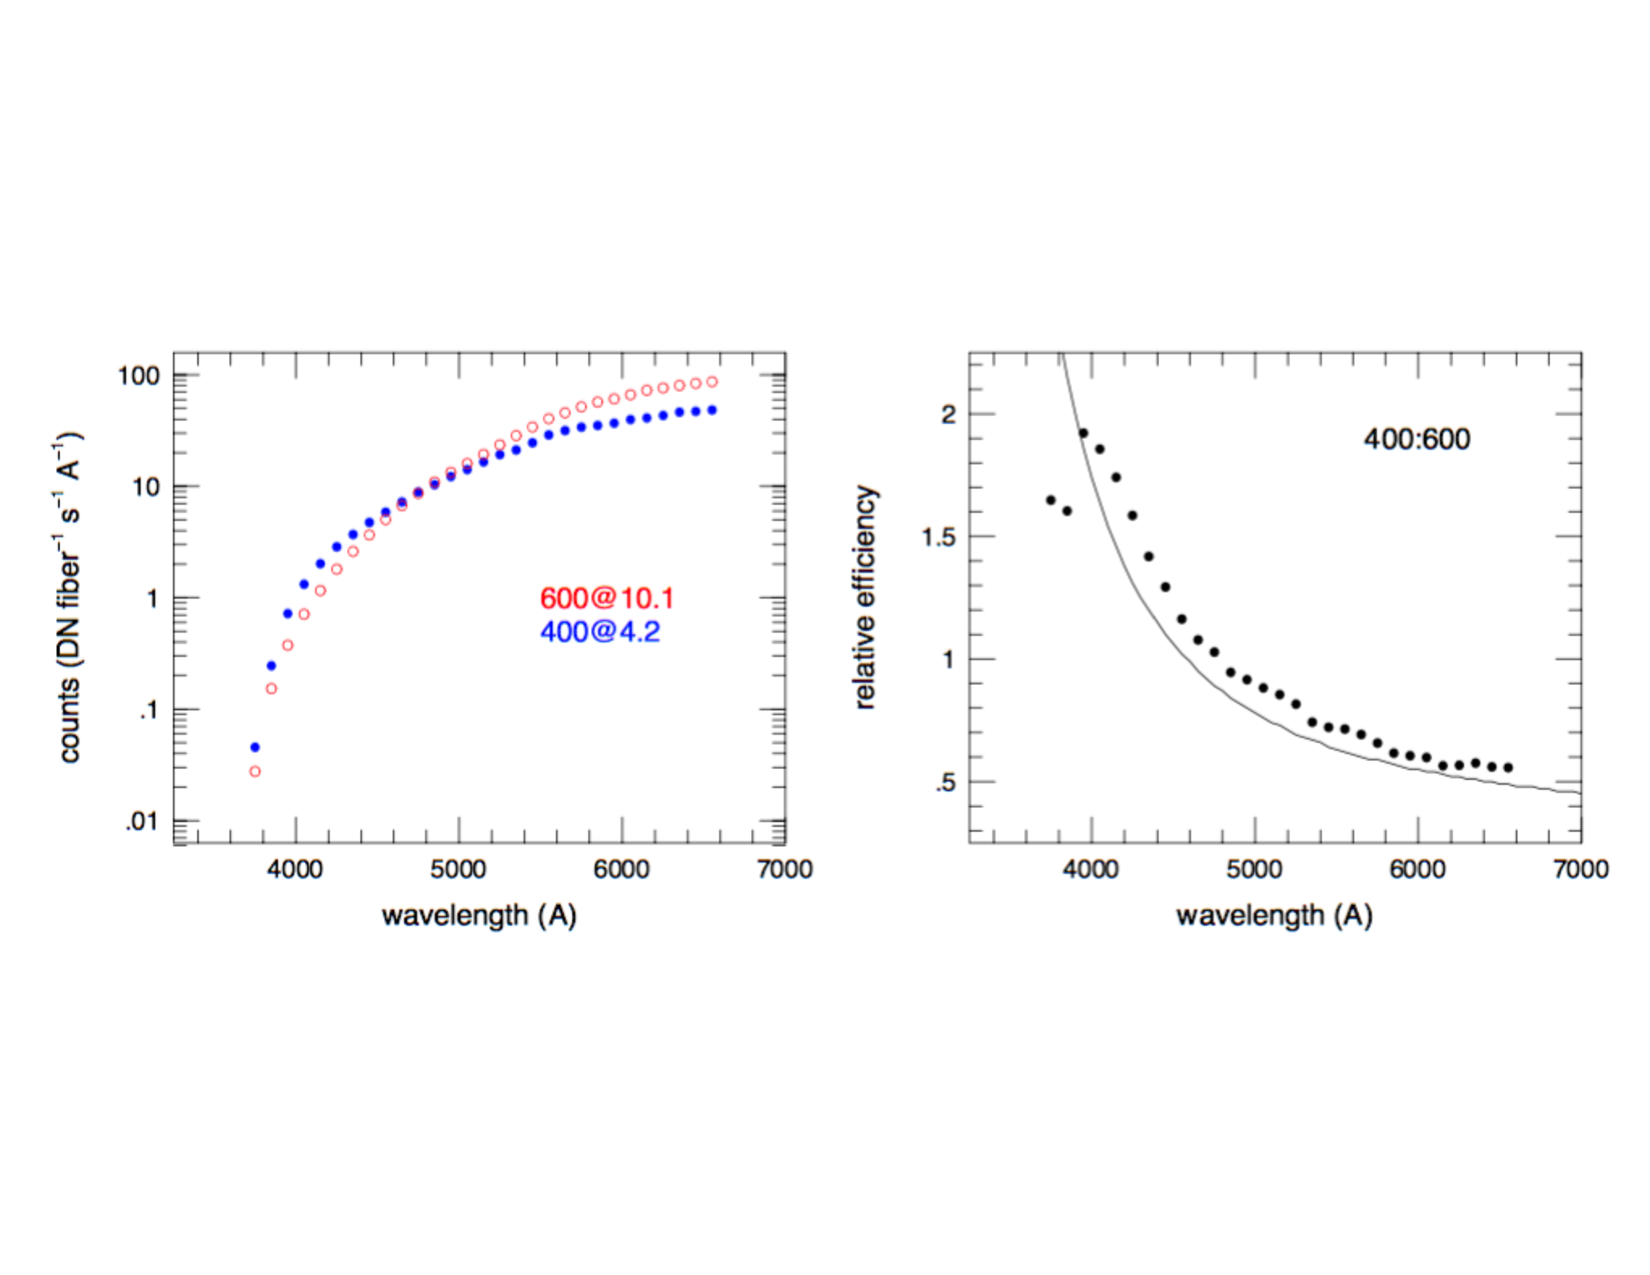
\includegraphics[width=\textwidth]{Appendix/figs/blaze_comp_land.pdf}
\vskip -1.25in
\caption[NGC 891 observing program grating
optimization]{\label{fig:grating_comp}\fixspacing Efficiency
  comparison between 400@4.2 and 600@10.1 gratings based on dome-flat
  exposures using the same fibers, spectrograph camera-collimator
  angle, and lamp temperature and intensity. Details are provided in
  text. The top panel shows counts for each grating, while the bottom
  panel shows their ratio and the prediction (line) based on the blaze
  functions for idealized gratings.}
\end{figure*}

% inferring camera fl. of 277.1mm,
% 400@4.2 with alpha=21.8 covers 3597-7867 A; blaze wave is 3496 A.
% 400@4.2 with alpha=21.53 covers 3372-7640 A; blaze wave is 3496 A.
% 600@10.1  with alpha=24.33 covers 3795-6657; blaze wave is 5666 A.

% Notes: effective camera fl at central waves of 5524 (g600) and 5733
% (g400) is 277.1 mm compared to nominal value of 285 mm. This is due to
% chromatic behvior of all-refractive camera and the ned to
% significantly modify focus for good image-quality across our primary
% bandpass.

% The band-pass in the plots can be shifted redward or bluerward with a
% commensurate shift (or offset) in the camera-collimator angle
% w.r.t. what is plotted here.

We chose the 400@4.2 grating out of the library of gratings available
on the WIYN Bench Spectrograph because it allows us to capture
simultaneously spectra from Ca H\&K to \Ha while still maintaining
relatively high efficiency at the blue end of the spectrum.  To
optimize our grating choice we compared the 400@4.2 grating to the
600@10.1 grating. The latter provides a narrower wavelength range but
at higher resolution, and, most importantly, the covered range is
marginally sufficient to meet our scientific objectives.  The 600@10.1
grating is often the ``go to'' grating for low-resolution programs
centered around \val{5500}{\AA}, particularly because it is the newest
reflection grating and purportedly has the highest diffraction
efficiency.

For testing during engineering time we compared the 400@4.2 grating
set to 21.8$^{\circ}$ and the 600@10.1 grating set to 24.33$^{\circ}$,
both for a fixed camera-collimator angle of 30$^{\circ}$ (this is the
nominal configuration for low-order gratings).\footnote{At these
  wavelengths the effective camera focal-length for this
  all-refractive compound optic is 277.1 mm not the nominal 285 mm
  quoted in reference manuals.} These grating incidence angles gave
wavelength ranges of \val{3600}{\AA}$< \lambda <$ \val{7867}{\AA} and
\val{3794}{\AA}$< \lambda <$ \val{6655}{\AA}, respectively. The blue
Hydra cable (300 $\mu$m core fibers) was used to observe dome flats
illuminated with identical lamp intensity (and temperature)
settings. The dome lamps are known to be stable to better than 10\%
over a broad wavelength range. Although we were concerned that
temperature instability might be a factor at the blue end of our
spectral range, our results are consistent with a highly stable
illumination over our full spectral range.

The fiber flux in the dome-flat spectra was measured on the raw
two-dimensional images before extraction. This was done in order to
exclude defocus effects from the fractional flux extracted along the
trace in wavelength, and between the two grating configurations for
which the detailed focus changes with wavelength are different.
Identical fibers and extraction regions were measured in both
configurations. The regions account for a small lateral shift along
the slit due to a slight difference in the alignment angle between
gratings orthogonal to the dispersion axis (this variance is just a
mechanical tolerance in the grating mount). Taking advantage of the
numerous broken Hydra fibers, we identified well-separated
transmitting fibers that had ample separation for extracting ``on''
and ``off'' signal regions (or apertures) at all wavelengths.  These
apertures were 10-11 pixels wide, and were adjacent on the CCD.  The
resulting counts were differenced and then scaled for the
corresponding exposure time and linear dispersion. 

Figure \ref{fig:grating_comp} shows the result of this experiment. It
is evident from the top panel that the 400@4.2 has greater efficiency
compared to the 600@10.1 grating blueward of 4700\AA. Since the
spectrograph configurations were identical except for the gratings,
under the assumption that the dome-flat illumination was constant, the
ratio of the two curves is equivalent to the ratio of the grating
blaze functions. As the bottom panel shows, this is very close to what
would be expected from simply computing the theoretical blaze
functions for idealized versions of these two gratings. If anything,
the 400@4.2 appears to have 10\% higher efficiency across all
wavelengths than the idealized case.

\begin{figure*}[htb]
  \centering
\vskip -1.25in
  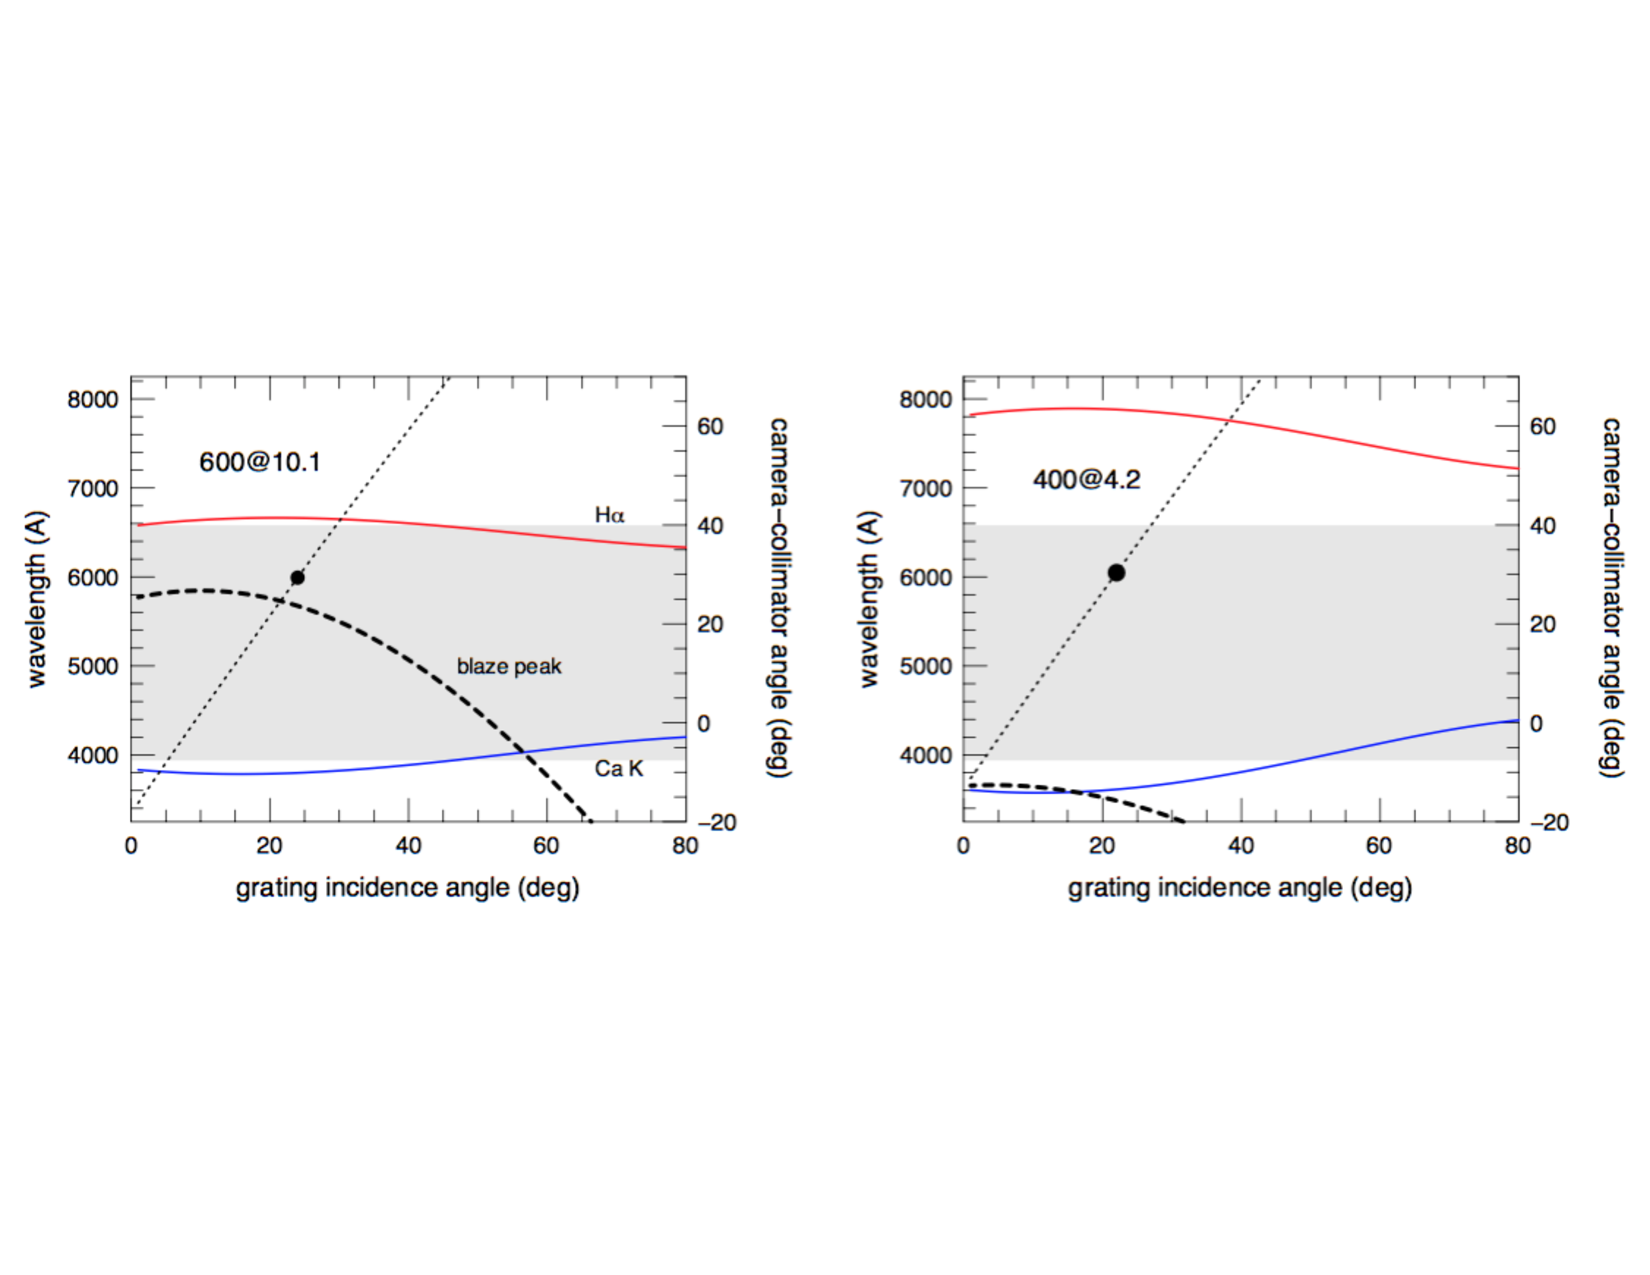
\includegraphics[width=\textwidth]{Appendix/figs/blaze_plot_land.pdf}
\vskip -1.25in
\caption[Comparison of coverage and blaze for 400 and 600 l/mm
gratings]{\label{fig:spec_config}\fixspacing Wavelength blaze and
  coverage for the Bench Spectrograph and the 400 l/mm grating blazed
  at 4.2 deg (top panel) and the 600 l/mm grating blazed at 10.1 deg
  (bottom panel) as a function of grating incidence angle and
  camera-collimator angle with the central wavelength held
  constant. Upper and lower wavelength limits and the blaze peak are
  marked with the red, blue, and thick-dashed lines, respectively. The
  minimal desired wavelength range between the most blue-shifted Ca-K
  line and most redshifted H$\alpha$ lines (3937-6480\AA; 300-800
  km/s) is shown as the grey shaded region The camera-collimator angle
  is marked with the thin dotted line, and corresponds to the
  right-hand vertical scale; the nominal value of 30 deg is marked
  with a dot.}
\end{figure*}

Since we are working with a bench-mounted spectrograph that in
principle is highly configurable, we also considered if additional
spectrograph layout modification might further optimize
performance. In particular, by altering both the grating (incidence)
angle and the camera-collimator angle, it is possible to change the
blaze wavelength while keeping the wavelength coverage on the detector
roughly constant. The concept is illustrated in \ref{fig:spec_config}.
The effect of increasing the camera-collimator angle for low-blaze
gratings shifts the blaze wavelength to the blue. This is not
desirable for the 400@4.2 grating which already has a very blue blaze
wavelength at the nominal camera-collimator angle of 30$^{\circ}$, but
this is potentially relevant for the 600@10.1 grating. Unfortunately,
significant shifts of the blaze wavelength require very large
camera-collimator angles that are both geometrically impractical on
the existing optical bench and lead to an unacceptable decrease in
spectral coverage. The exercise does conclude that a larger
camera-collimator angle of roughly 40$^{\circ}$ would be preferable
for the 600@10.1 grating, but its performance in the far blue would
still fall short of the 400@4.2 grating.